\scanpage{44}
Ici, prenant les top. étales sur les préschémas, et les faisceaux \unsure{cts} $A_X$ $(\mathbf{Z}/n\mathbf{Z}=A)$, tous les morphismes de topoi annelés envisagés sont plats.

\figure{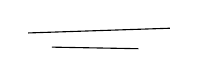
\begin{tikzpicture}\draw (0,0)--(1.8,.06);\draw (.3,-.18)--(1.4,-.2);\end{tikzpicture}}

\diagram{\begin{tikzcd}
\unsure{F}&\\[-15pt]
X\arrow[d,"f"',no head]&X'\arrow[l,"h"']\arrow[d,"f'"]\\
Y&Y'\arrow[l,"g"']
\end{tikzcd}}
Si $f$ quelconque, on définit pour $F^\cdot\in\operatorname{Ob}D^+(X)$ un hom (dans la catégorie dérivée $D^+(Y')$)
\[
(*)\qquad \deleted{Rf'_*(h^*F^\cdot)\longleftarrow}\boxed{g^*(Rf_*(F^\cdot))\longrightarrow Rf'_*(h^*(F^\cdot))}.
\]
Passant aux faisceaux de \unsure{coh.}, cela redonne
\[
(*_i)\qquad g^*R^if_*(F))\longrightarrow R^if'_*(h^*(F)))
\]
\uline{Lorsque} $f$ \uline{est propre} ce sont des isom, puisque on sait que les $(*_i)$ le sont.
\mspage{43}
